\documentclass{article}

\usepackage{graphicx}
\usepackage{tikz}
\usepackage{tikzsymbols}
\usetikzlibrary{calc,patterns,shapes.geometric}
\pagestyle{empty}
\usepackage[margin=0pt]{geometry}
\geometry{papersize={14in,12in}}

\def\centerarc[#1](#2)(#3:#4:#5){\draw[#1] ($(#2)+({#5*cos(#3)},{#5*sin(#3)})$) arc (#3:#4:#5);}

\begin{document}
	\begin{figure}
		\centering
		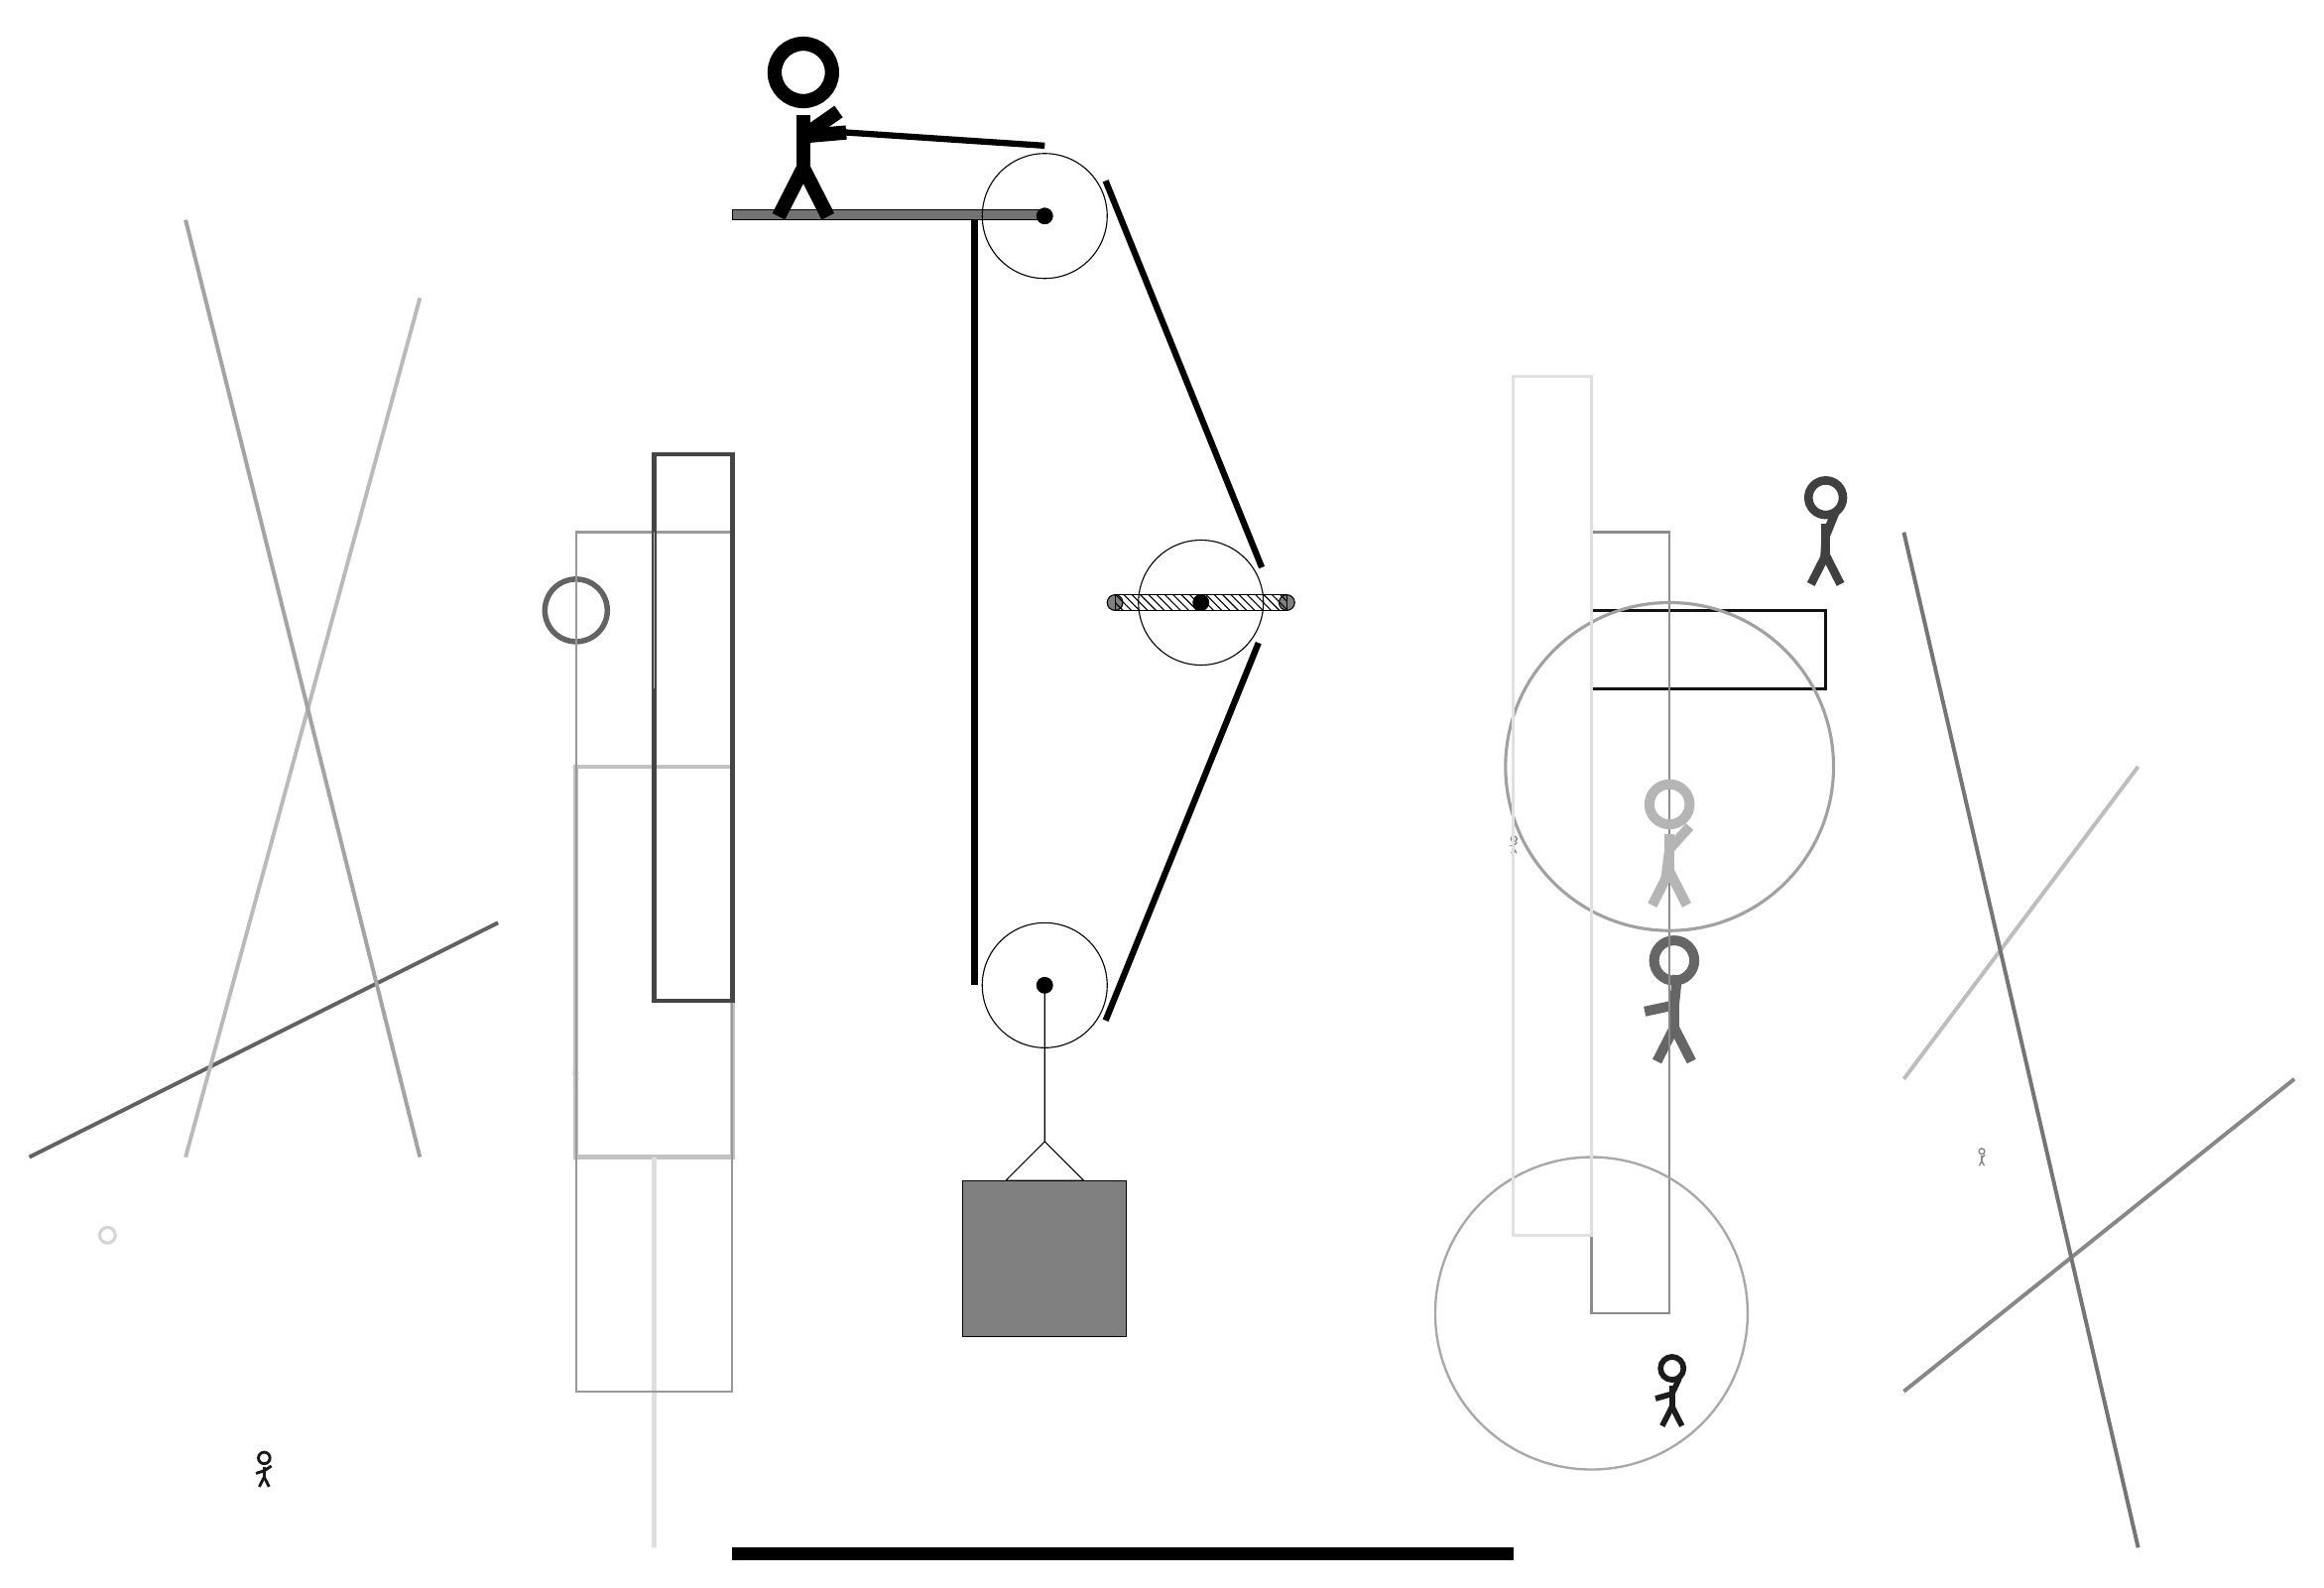
\begin{tikzpicture}
			%%%%% START %%%%%
			
			\draw[fill=black!55] (-2, 14) rectangle (2, 14.125);
			
			\draw (2, 4.2) circle (0.8);
			\draw[fill=black] (2, 4.2) circle (0.1);
			
			\draw (2, 14.05) circle (0.8);
			\draw[fill=black] (2, 14.05) circle (0.1);
			
			\draw [line width=0.7mm, color=black!61](-4, 9) circle (0.4);
			
			\node[line width=0.5mm, color=black!47] at (8, 6) {\Strichmaxerl[1][0][43]};
			\node[line width=0.2mm, color=black!11] at (-4, 3) {\Strichmaxerl[1][78][10]};
			\draw[line width=0.5mm, color=black!47](13, -1) -- (18, 3);
			\draw[line width=0.6mm, color=black!24] (-4, 7) rectangle (-2, 2);
			\draw[line width=0.4mm, color=black!93] (9, 9) rectangle (12, 8);
			
			\draw[line width=0.5mm, color=black!26](13, 3) -- (16, 7);
			
			\node[line width=0.5mm, color=black!75] at (12, 10) {\Strichmaxerl[6][87][68]};
			\draw[line width=0.5mm, color=black!54](13, 10) -- (16, -3);
			\node[line width=0.5mm, color=black!60] at (10, 4) {\Strichmaxerl[7][12][84]};
			
			\draw[line width=0.6mm, color=black!13] (-3, 2) rectangle (-3, -3);
			\draw[line width=0.3mm, color=black!45] (10, 10) rectangle (9, 0);
			\node[line width=0.6mm, color=black!47] at (14, 2) {\Strichmaxerl[1][89][43]};
			
			\draw[line width=0.3mm, color=black!40] (-4, 10) rectangle (-2, -1);
			\draw[line width=0.5mm, color=black!62](-5, 5) -- (-11, 2);
			\draw [line width=0.3mm, color=black!34](9, 0) circle (2.0);
			
			\draw[line width=0.5mm, color=black!27](-6, 13) -- (-9, 2);
			
			\draw[line width=0.6mm, color=black!73] (-2, 11) rectangle (-3, 4);
			\node[line width=0.5mm, color=black!90] at (-8, -2) {\Strichmaxerl[2][18][33]};
			\draw [line width=0.4mm, color=black!37](10, 7) circle (2.1);
			\draw[line width=0.4mm, color=black!12] (9, 12) rectangle (8, 1);
			
			\draw[line width=0.5mm, color=black!36](-6, 2) -- (-9, 14);
			
			\node[line width=0.4mm, color=black!29] at (10, 6) {\Strichmaxerl[7][83][48]};
			\draw[line width=0.2mm, color=black!29] (-3, 10) rectangle (-3, 8);
			\node[line width=0.2mm, color=black!89] at (10, -1) {\Strichmaxerl[4][16][65]};
			\draw [line width=0.4mm, color=black!17](-10, 1) circle (0.1);
			
			\draw[fill=white](4, 9.1) circle (0.8);
			\draw[fill=black] (4, 9.1) circle (0.1);
			\draw[fill=black!50] (2.9, 9.1) circle (0.1);
			\draw[fill=black!50] (5.1, 9.1) circle (0.1);
			\draw[pattern=north west lines, pattern color=black] (2.9, 9.2) rectangle (5.1, 9.0);
			
			\draw (2, 4.2) -- (2, 2.2) -- (1.5, 1.7) -- (2.5, 1.7) -- (2, 2.2);
			\draw[fill=black!50] (0.95, 1.7) rectangle (3.05, -0.3);
			
			\draw[line width=0.8mm] (1.1, 14) -- (1.1, 4.2);
			\centerarc[line width=0.8mm](2, 4.2)(180:330:0.9);
			\draw[line width=0.8mm](2.7794, 3.75) -- (4.7373, 8.5838);
			\centerarc[line width=0.8mm](4, 9.1)(390:325:0.9);
			\draw[line width=0.8mm](4.7794, 9.55) -- (2.7794, 14.5);
			\centerarc[line width=0.8mm](2, 14.05)(30:90:0.9);
			\draw[line width=0.8mm](2, 14.95) -- (-1, 15.15);
			
			\node at (-1, 15.15) {\Strichmaxerl[10][-175][35]};
			
			\draw[fill=black] (-2, -3) rectangle (8, -3.15);
			
			%%%%% END %%%%%
		\end{tikzpicture}
	\end{figure}	
\end{document}